\documentclass[tikz, border=1mm]{standalone}

\usepackage{pgfplots}
\pgfplotsset{compat=1.15}
\usepackage{mathrsfs}
\usepackage{amsfonts}
\usetikzlibrary{arrows}
\pagestyle{empty}


\begin{document}

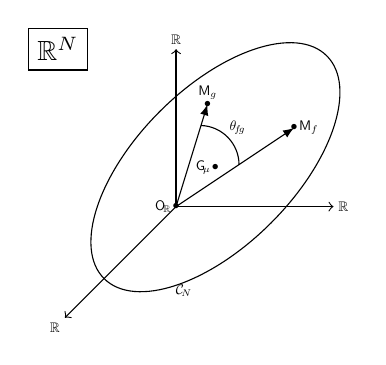
\begin{tikzpicture}

% Write
\node[draw] at (-1.5, 2) {$\mathbb{R}^N$};

% Axis
\draw[->] (0, 0) -- (2, 0);
\draw (2, 0) node[right, scale=0.5] {$\mathbb{R}$};

\draw[->] (0, 0) -- (0, 2);
\draw (0, 2) node[above, scale=0.5] {$\mathbb{R}$};

\draw[->] (0, 0) -- (-1.412, -1.412);
\draw (-1.412, -1.412) node[below left, scale=0.5] {$\mathbb{R}$};

% Points
\draw (0, 0) node[scale=0.5] {$\bullet$};
\draw (0, 0) node[left, scale=0.5] {$\mathsf{O}_{\!\mathbb{R}}$};

\draw (0.5, 0.5) node[scale=0.5] {$\bullet$};
\draw (0.5, 0.5) node[left, scale=0.5] {$\mathsf{G}_{\!\mu}$};

\draw (1.5, 1) node[scale=0.5] {$\bullet$};
\draw (1.5, 1) node[right, scale=0.5] {$\mathsf{M}_f$};

\draw (0.4, 1.3) node[scale=0.5] {$\bullet$};
\draw (0.4, 1.3) node[above, scale=0.5] {$\mathsf{M}_g$};


% Limes
\draw[->, >=latex] (0, 0) -- (1.5, 1);
\draw[->, >=latex] (0, 0) -- (0.4, 1.3);

% Arc
\draw (0.8, 0.53) arc (0:88:0.5);
\draw (0.78, 0.85) node[above, scale=0.5] {$\theta_{\!f\!g}$};

% Cloud
\draw[rotate around={45:(0.5, 0.5)}] (0.5, 0.5) ellipse (2cm and 1cm);
\draw (0.1, -1.2) node[above, scale=0.5] {$\mathcal{C}_{\!N}$};

% Distance


\end{tikzpicture}

\end{document}